\begin{figure}[t]
    \centering
    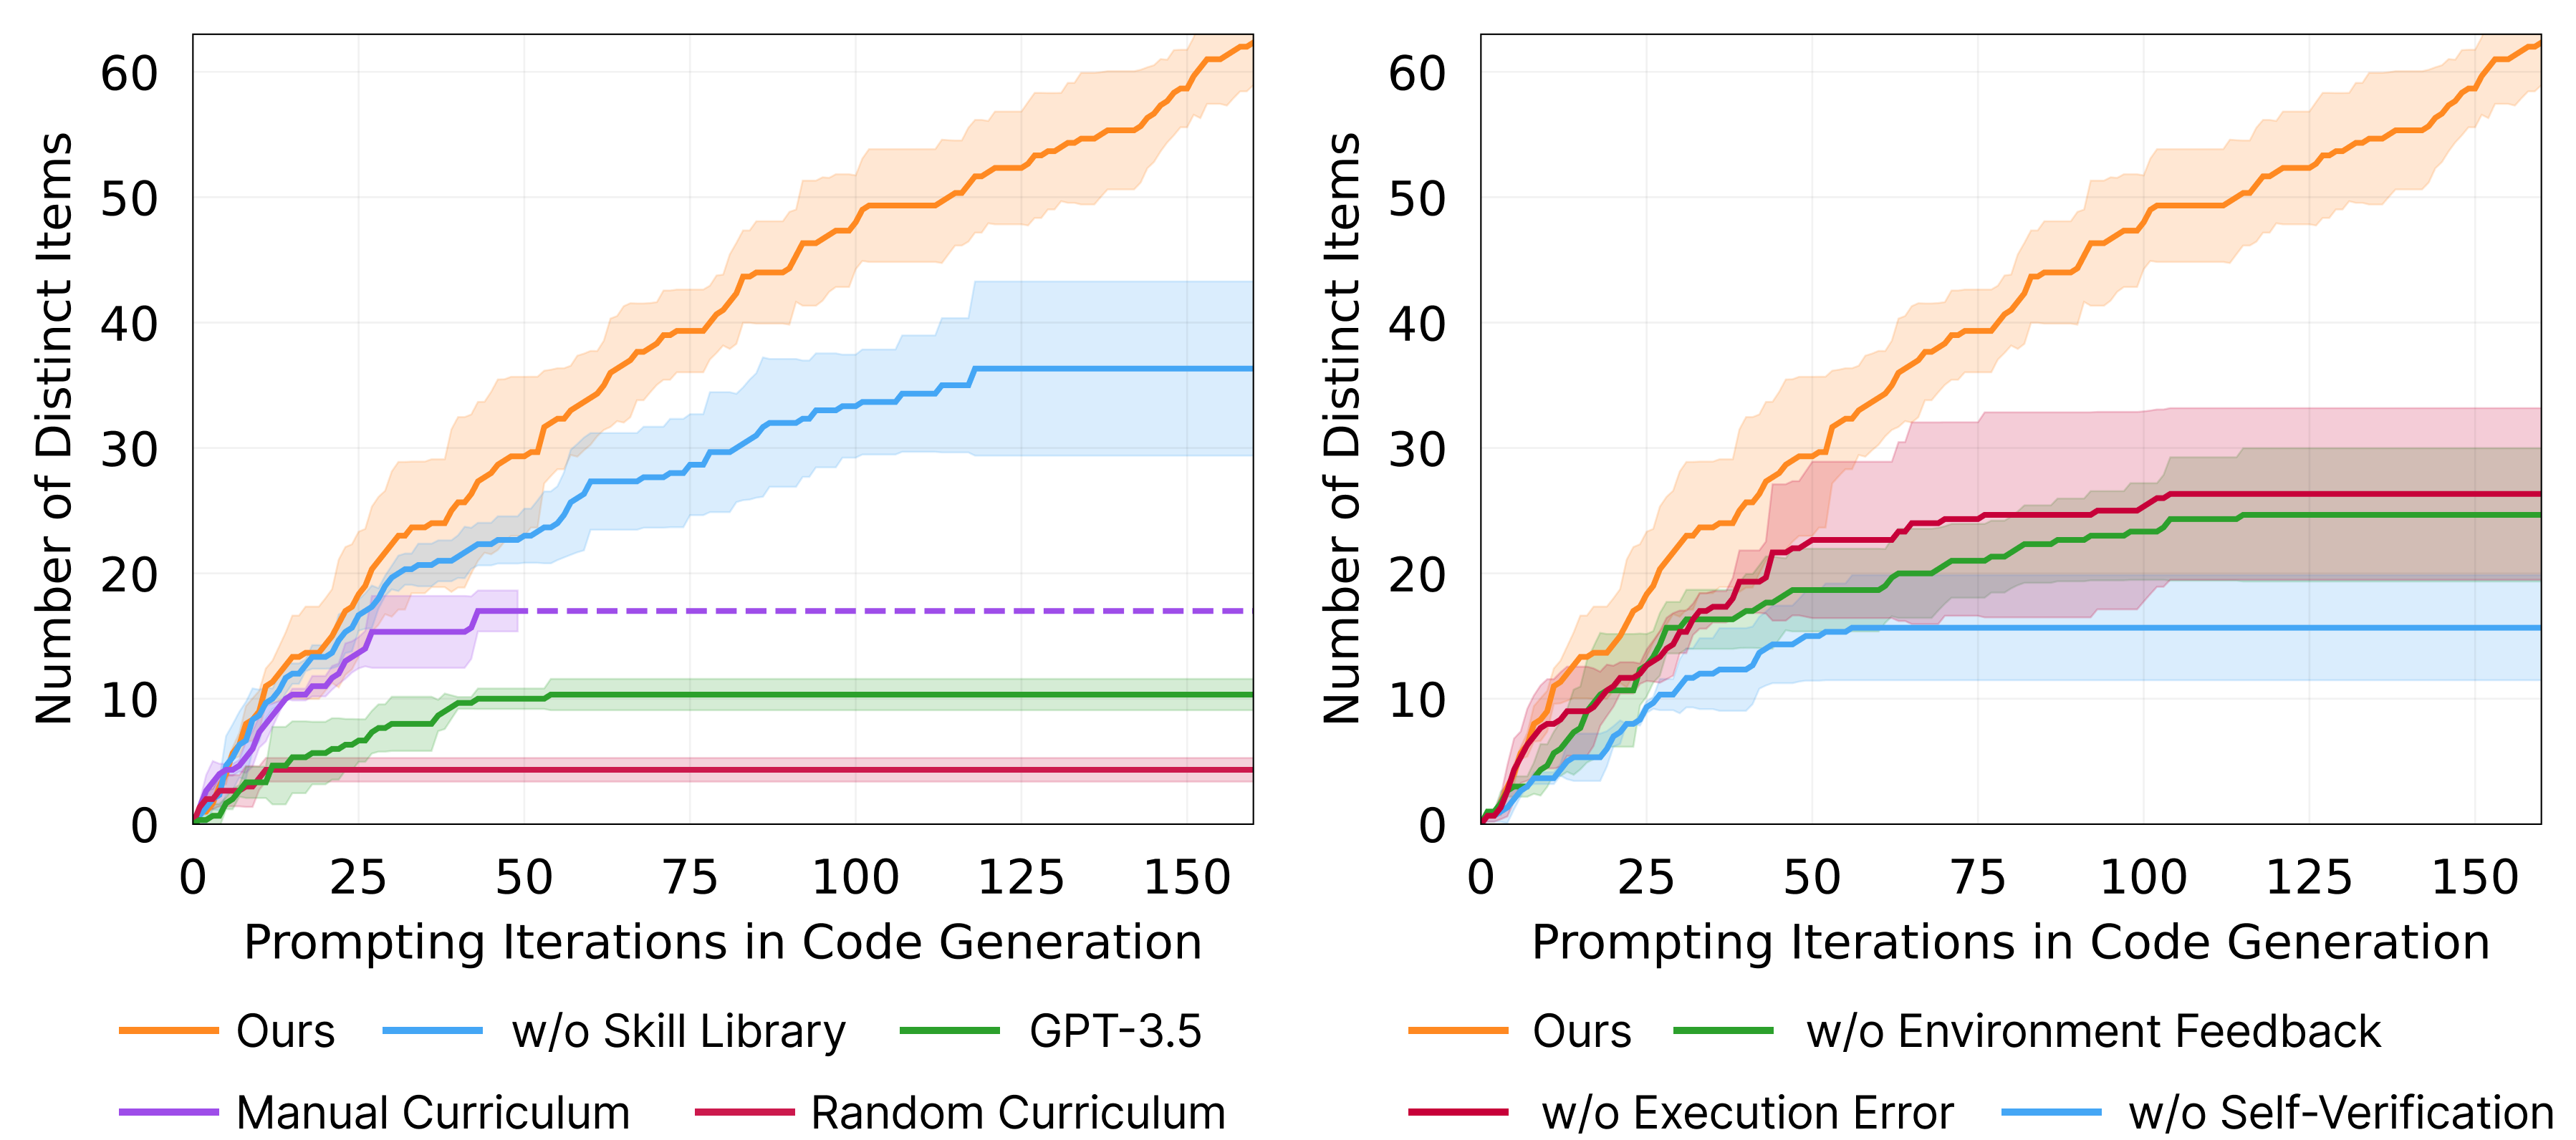
\includegraphics[width=0.8\textwidth]{figures/ablation_fig.png}
    \caption{\textbf{Left: Ablation studies for the automatic curriculum, skill library, and GPT-4.} GPT-3.5 means replacing GPT-4 with GPT-3.5 for code generation. \voyager outperforms all the alternatives, demonstrating the critical role of each component. \textbf{Right: Ablation studies for the iterative prompting mechanism.} \voyager surpasses all the other options, thereby highlighting the essential significance of each type of feedback in the iterative prompting mechanism.}
    \label{fig:ablation}
\end{figure}